\documentclass[aspectratio=43]{beamer}

\usetheme{Padova}
\usepackage[utf8x]{inputenc}
\usepackage{listings}
\usepackage{wrapfig}

\usepackage{tikz,xparse}
\usetikzlibrary{decorations.pathreplacing,}
\newcommand{\tikzmark}[1]{\tikz[baseline={(#1.base)},overlay,remember picture] \node[outer sep=0pt, inner sep=0pt] (#1) {\phantom{A}};}

%% syntax
%%%\mybrace{<first>}{<second>}[<Optional text>]
\NewDocumentCommand\mybrace{mmo}{%
\IfValueTF {#3}{%
\begin{tikzpicture}[overlay, remember picture,decoration={brace,amplitude=1ex}]
  \draw[decorate,thick] (#1.north east) -- (#2.south east) node[midway, right=0.1cm] {$=$}node[midway, right=0.5cm,text=grigioPantano,text width = 1.5in,] {{#3}};
\end{tikzpicture}%
}%
{%
\begin{tikzpicture}[overlay, remember picture,decoration={brace,amplitude=1ex}]
  \draw[decorate,thick] (#1.north east) -- (#2.south east);
\end{tikzpicture}%
}%
}%

\usepackage{subfigure}

\title{PICAT \\Analisi del linguaggio}
\author{Marco Zanella - 1155185}
\date{22 marzo 2017}


\begin{document}
	\maketitle
	\iffalse
PICAT è un linguaggio di programmazione creato da un professore di informatica Neng-Fa Zhou di Brooklyn e il nome è una sigla che significa Pattern-matching Intuitive Constraint Actors Tabling
* Pattern Matching perchè il linguaggio permette di definire funzioni o predicati utilizzando appunto il pattern matching
* Intuitive perchè secondo l'ideatore è stato creato cercando di avvicinare il più possibile il linguaggio a quello che si vuole modellare, anche grazi l'introduzione di costrutti di vari tipi di programmazione come i loop della programmazione imperativa oppure la list comprehension tipica dei linguaggi funzionali
* Constaint perchè supporta la programmazione con vincoli e poichè prevede 3 moduli chiamati cp, sat e mip per la soluzione di questo tipo di problemi
* Actor perchè permette la programmazione event driven ***COME SI FA CHE NON HO TROVATO MATERIALE DECENTE?***
* Tabling perchè il linguaggio ha delle primitive che permettono di effettuare la memoizzazione di risultati senza dover ricalcolarli ogni volta
Come si capisce anche dal significato del nome questo linguaggio è stato influenzato da differenti altri linguaggi, supporta differenti paradigmi di programmazione
È stato modellato per essere un linguaggio di scripting utile soprattutto in problemi di intelligenza artificiale, per la risoluzione di sistemi di vincoli, problemi di pianificazione o programmazione dinamica
È un linguaggio abbastanza recente(2013 e l'ultima release è la versione 2.1 di quest'anno) e poco conosciuto tant'è che ha una entry su wikipedia solamente in italiano e che nelle prime 100 posizioni dell'indice TIOBE non è presente
\fi

\begin{frame}{Informazioni generali}

	\begin{columns}
		\begin{column}{0.8\textwidth}
			\begin{itemize}
				\item Pattern-matching Intuitive Constraints Actors Tabling
				\item Creato da Neng-Fa Zhou, professore di informatica del Brooklyn College
				\item Pensato per risolvere problemi di intelligenza artificiale
					\begin{itemize}
						\item Influenzato da differenti linguaggi
						\item Implementa differenti paradigmi di programmazione
					\end{itemize}
			\end{itemize}
		\end{column}

		\begin{column}{0.3\textwidth}
			
			\begin{figure}
				\centering
				
\includegraphics[scale=2.5]{res/picatLogo}
			\end{figure}

			\begin{figure}
				\centering
				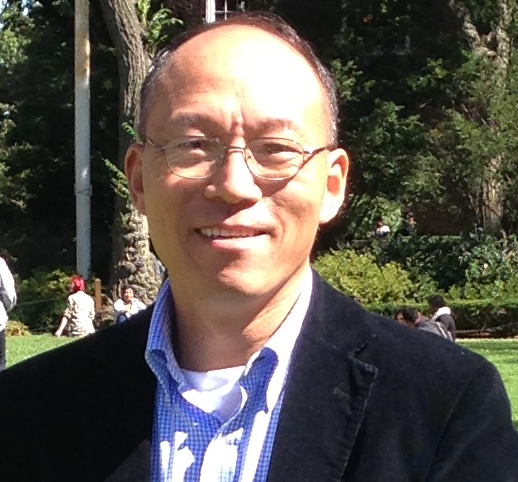
\includegraphics[scale=0.22]{res/zhou}
			\end{figure}
		
		\end{column}
	\end{columns}

\end{frame}
	\iffalse
Ora introdurrò alcune caratteristiche di PICAT generali e poi parlerò di alcuni dei paradigmi di programmazione che supporta, confrontandolo con altri linguaggi.

PICAT è un linguaggi dynamically typed e la maggior parte dei suoi tipi sono uguali a quelli del prolog ad eccezione di array e liste.
Le variabili devono o iniziare con la lettere maiuscola oppure con l'underscore come in prolog
I tipi di base sono solamente i caratteri e i numeri che possono essere o interi o reali
Poi ci sono i tipi composti:
- le liste sono rappresentate internamente come delle liste singolarmente linkate la lui lunghezza non è salvata ma viene ricalcolata ogni volta e sono rappresentate tramite le parentesi quadre
- le stringhe sono rappresentate solamente come delle liste di carattari
- le strutture sono rappresentate come dollaro-nome-grafa-parametri-grafa
- gli array sono delle strutture senza nome. A differenza delle liste per gli array ne viene salvata la lunghezza (così è possibile accedervi in tempo costante come è possibile accedere all'elemento in pos i in tempo costante)
PICAT prevede sia list che array comprehension e per tutti questi tipi è possibile l'index notation per accedere agli elementi
Gli altri tipi compound sono la mappa che è una normale tabella chiave valore mentr il set è una mappa di sole chiavi
\fi

\begin{frame}{Overview - Tipi}
	
	\begin{figure}
		\centering
		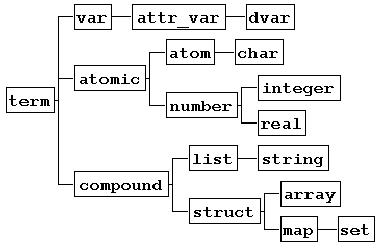
\includegraphics[scale=1]{res/tipi}
	\end{figure}

\end{frame}
	\iffalse
Qui possiamo vedere un po' di esempi per la creazione di array, liste, strutture e mappe
Liste e array possono essere creati elencando gli elementi, con new_list e new_array oppure con list e array comprehension
Per creare le strutture invece è necessario anteporre il dollaro prima del nome della struttura per far capire al sistema che non si tratta di una chiamata di funzione
le mappe si creano con la funzione new_map e poi è possibile inserire gli elementi con la funzione put e ricavarli invece con la funzione get. Nel caso venga richiesto il get da una mappa senza che tale chiave sia presente allora viene lanciata una eccezione, per evitarlo è possibile aggiungere un valore di default quando si fa la chiamata
\fi

\begin{frame}[fragile, shrink=1]{Overview - Creazione oggetti compound}
	
	\begin{lstlisting}
%Esempi per la creazione di una lista
Picat>X=[a,b,c],Y=new_list(3),Z=[Z:Z in 1..6,even(Z)]
X = [a,b,c]
Y = [_104c8,_104d8,_104e8]
Z = [2,4,6]
%Esempi per la creazione di un array
Picat>X={a,b,c},Y=new_array(3),Z={Z:Z in 1..6,even(Z)}
X = {a,b,c}
Y = {_1b220,_1b228,_1b230}
Z = {2,4,6}
%Esempio di struttura
Picat>X = $str(abc, 1000, a), Y=X[1]
X = str(abc,1000,a)
Y = abc
%Esempio con una mappa
Picat>X=new_map(),X.put(1, a),X.put(2, b),Y=X.get(1)
X = (map)[1 = a,2 = b]
Y = a
	\end{lstlisting}

\end{frame}
	\iffalse
Una della particolarità di questo linguaggio è la presenza di tre tipi di mappe globali. Tali mappe permettono di salvare dei valori e di accedervi ovunque nel codice.
La prima è la heap map, che viene costruita sullo heap. Per questo tipo di mappa in caso di predicati che prevedono il backtracking il risultato viene aggiornato
La seconda e la terza invece sono global map e la table map, che vengono create in un area di memoria globale dove picat viene lanciato. La differenza tra i due è che la table map utilizza l'hash consing, ovvero al posto di memorizzare valori uguali ne viene solamente salvato un riferimento, in modo da avere un miglioramente di prestazioni in tempo e spazio
È possibile creare differenti istanze di queste mappe globali associando ad ognuna di esse un identificativo, con il quale anche è possibile accedervi
\fi

\begin{frame}[fragile, shrink=1]{Overview - Global maps}

	Presenza di tre tipi di mappe globali:
	\begin{itemize}
		\item heap map
		\item global map \tikzmark{a}
		\item table map\hspace{0.15cm}  \tikzmark{b}
	\end{itemize}
\mybrace{a}{b}[No aggiornamento in caso di backtracking]

	\begin{lstlisting}
%Esempio di utilizzo
fun() =>
	X = get_global_map(0),
	println(X.get(2)),
	X.put(1, val1modified).
main =>
	X = get_global_map(0),
	X.put(1, val1),X.put(2,val2),X.put(3,val3),
	fun(),
	println(X.get(1)).
	\end{lstlisting}
\end{frame}
	\iffalse
Come già anticipato PICAT è un linguaggio multiparadigma, ed è stato influenzato da differenti linguaggi, sopratutto da Prolog. Inoltre è stato modellato come un linguaggi di scripting, prendendo anche come esempio Python.
\fi

\begin{frame}{Molte influenze}

	Implementa differenti paradigmi di programmazione
	\begin{itemize}
		\item Programmazione logica
		\item Programmazione imperativa
		\item Programmazione funzionale
	\end{itemize}

	\vspace{1em}
	Pensato come linguaggio di scripting

	\begin{figure}
		\centering
		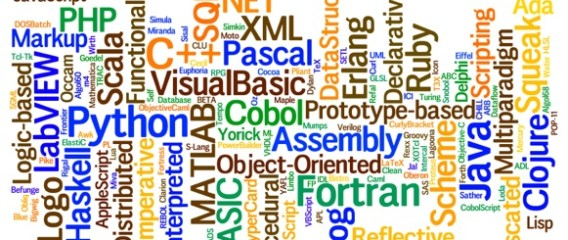
\includegraphics[scale=0.4]{res/influenze}
	\end{figure}
\end{frame}
	\iffalse
Della programmazione logica troviamo delle caratterisctiche tipiche come la possibilità di definire le relazioni, la possibilità di definire predicati e di farne backtracking (quindi abbiamo il non determinismo) ed infine è presente l'operatore di unificazione.

*** AGGIUNGERE ESEMPI ***
\fi

\begin{frame}[fragile]{Programmazione logica}

	\begin{itemize}
		\item Regole per definire relazioni
		\item Predicati
			\begin{itemize}
				\item Senza backtraking: \\\hspace{1cm} \texttt{Head, Cond $\Rightarrow$ Body}
				\item Con backtracking: \\\hspace{1cm} \texttt{Head, Cond ?$\Rightarrow$ Body}
			\end{itemize}
		\item Operatore di unificazione
		\item Tabling
	\end{itemize}

\end{frame}
	\iffalse
PICAT come linguaggi è molto simile al Prolog e difatti la prima versione di questo linguaggio riutilizza molto del codice di B-Prolog, quindi ha senso confrontare questi due linguaggi.
Una delle differenze più importanti è che in PICAT il non determinismo deve essere previsto esplicitamente da chi scrive un determinato predicato, mentre in Prolog tutti i predicati prevedono implicitamente il backtracking (se si vuole controllare il backtracking è necessario utilizzare l'operatore cut).
Un'altra differenza è che in PICAT la scelta del predicato da chiamare non viene fatta attraverso l'operatore di unificazione come in Prolog, bensì utilizzando il pattern matching.
L'ultima importante è sui costrutti: infatti PICAT prevede costrutti tipici della programmazione imperativa e funzionale, come cicli, array e list comprehension,l'assegnazione, e ciò permette di esprimere più facilmente alcuni concetti
\fi

\begin{frame}[fragile]{PICAT vs Prolog}

	\begin{columns}

		\begin{column}{1\textwidth}
			Analogie
			\begin{itemize}
				\item Prima versione di PICAT è basata sul codice di B-Prolog
				\item Condividono molti aspetti della programmazione logica
				\item Tipi
				\item Sintassi
			\end{itemize}

			Differenze
			\begin{itemize}
				\item Non determinismo esplicito
				\item Scelta del predicato avviene tramite pattern matching
				\item Presenza di più costrutti
					\begin{itemize}
						\item Cicli
						\item Array e list comprehension
						\item Assegnazione
						\item Funzioni
					\end{itemize}
			\end{itemize}

		\end{column}

		\begin{column}{0.1\textwidth}
			\begin{figure}
				\vspace*{4cm}
				\hspace*{-3.5cm}
				
\includegraphics[scale=0.2]{res/prologLogo}
			\end{figure}
		\end{column}

	\end{columns}

\end{frame}


	\iffalse
Oltre alla programmazione logica, PICAT è pensato anche per implementare la programmazione imperativa. Di questa possiede alcuni caratteristiche tipiche come l'assegnazione, oppure costrutti che riguardano il control flow quindi l'if-then-else ed i cicli. 
\fi

\begin{frame}{Programmazione imperativa - 1}

	\begin{columns}
		\begin{column}{0.5\textwidth}
			\begin{itemize}
				\item Assegnazione e side-effects
				\item If-Then-Else
				\item Cicli
				\begin{itemize}
					\item foreach
					\item while
				\end{itemize}
			\end{itemize}
		\end{column}

		\begin{column}{0.5\textwidth}
			
			\begin{figure}%
				\centering
				\subfigure{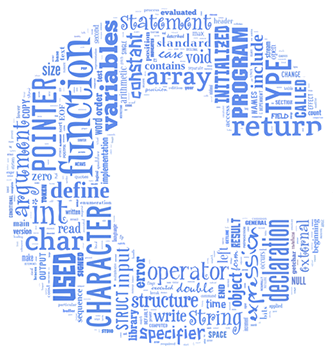
\includegraphics[scale=0.09]{res/cLogo}}\qquad
				\subfigure{
\includegraphics[scale=0.24]{res/c++Logo}}\\
				\subfigure{
\includegraphics[scale=0.03]{res/javaLogo}}%
			\end{figure}

		\end{column}
	\end{columns}

\end{frame}
	\iffalse
PICAT prevede costrutti di differenti paradigmi di programmazione anche perchè, quando è stato creato, l'autore aveva in mente che potesse essere un ponte tra i linguaggi imperativi nei quali il programmatore deve dire al computer cosa deve fare e i linguaggi dichiarativi, nei quali invece viene descritto cosa si vuole come risultato
\fi

\begin{frame}{Programmazione imperativa - 2}

	\textit{"The purpose of Picat is to bridge the gap between imperative languages, 
	which tell the computer how things should be done, and declarative 
	languages, which tell the computer what to do, without detailing how it 
	should be done"}

\end{frame}
	\iffalse
Qui possiamo vedere un esempio di programma in stile imperativo scritto in PICAT. Il programma inizia dal main con una lista vuota X e un numero I pari a zero. Poi viene fatto un wile inizializzando la lista e incrementando ad ogni ciclo I. Finito il ciclo viene richiamata la funzione prova modifica la lista.
Poi la lista viene riassegnata e ancora modificata con la funzione prova
\fi

\begin{frame}[fragile, shrink=20]{Programmazione imperativa - Esempio}

	\lstinputlisting{../examples/imperativeProgramming.pi}

\end{frame}
	\iffalse
PICAT inoltre prevede anche alcuni aspetti funzionali. A parte permettere la definizione di funzioni ricorsive, queste possono essere definite tramite l'utilizzo di pattern matching. Oltre a ciò PICAT prevede una serie di funzioni già pronte per la manipolazione delle liste ed una certa facilità a modificarle. PICAT prevede inoltre un limitato supporto alle funzioni higher order: non se ne possono creare di nuove infatti, come in un qualsiasi linguaggi funzionale, ma ne prevede un insieme già creato. L'uso di queste funzioni è scoraggiato nel caso in cui si voglia creare programmi efficienti poichè creano un overhead elevato
\fi

\begin{frame}{Programmazione funzionale}

	\begin{figure}
		\hfill
		
\includegraphics[scale=0.1]{res/lambda}
	\end{figure}

	\begin{itemize}
		\item Funzioni ricorsive
		\item Pattern matching per la definizione di funzioni
		\item Facilità a manipolare le liste (funzioni built-in e comprehension)
		\item Limitato supporto alle funzioni higher-order
			\begin{itemize}
				\item \texttt{apply}, \texttt{call}, \texttt{foldl}, \texttt{map}...
				\item Uso scoraggiato a causa dell'overhead elevato
			\end{itemize}
	\end{itemize}

	\begin{figure}
		\hspace*{-7cm}
		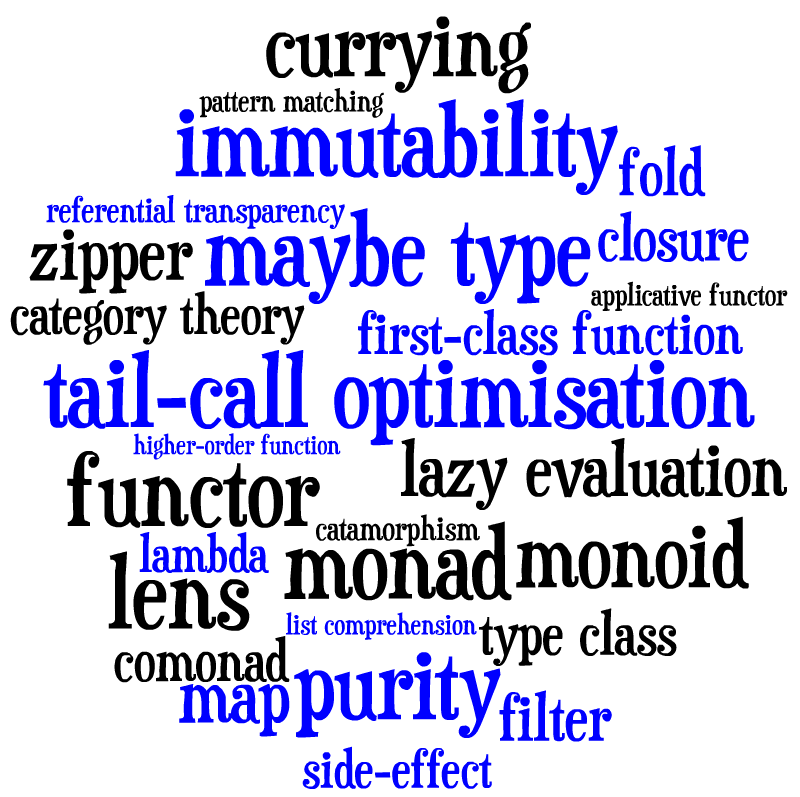
\includegraphics[scale=0.1]{res/functional}
	\end{figure}

\end{frame}
	\iffalse
Poichè PICAT presenta alcune funzionalità riconducibili ai linguaggi lo possiamo confrontare con un linguaggio prettamente funzionale come Haskell. Le analogie tra i due linguaggi sono praticamente tutti gli aspetti funzionali di PICAT ovvero: pattern matching, list comprehension, funzioni higher order che però in PICAT sono sconsigliate mentre in haskell ovviamente no ed in entrambi i linguaggi i side effects sono scoraggiati.
Le differenze sono che nel il primo è staticamente tipato a differenza del secondo: in haskell infatti quando viene eseguito un programma tutto ha un certo tipo mentre in PICAT è possibile riassegnare una certa variabile a tipi differenti.
Infine PICAT non prevede l'utilizzo della lazy evaluation, che permette per esempio ad haskell di gestire liste infinite, mentre PICAT no, infatti ogni termine deve essere completamente valutato per esempio prima di essere passato come parametro ad una funzione. Comunque è possibile in qualche modo simularla tramite il costrutto freeze che permette di posticipare la valutazione di un termine
\fi

\begin{frame}{PICAT vs Haskell - 1}
	
	\begin{columns}

		\begin{column}{1\textwidth}

			Analogie
			\begin{itemize}
				\item Funzioni definite con pattern matching
				\item Supporto funzioni higher order (call, apply, map, foldl...)
				\item List comprehension
				\item Side effect scoraggiati
			\end{itemize}

			Differenze
			\begin{itemize}
				\item Dinamicamente tipato
				\item No lazy evaluation
				\item L'utilizzo delle funzioni higher order è scoraggiato
			\end{itemize}

		\end{column}

		\begin{column}{0.1\textwidth}
			\begin{figure}
				\vspace*{-5cm}
				\hspace*{-2cm}
				
\includegraphics[scale=0.1]{res/haskellLogo}
			\end{figure}
		\end{column}

	\end{columns}
	
\end{frame}


	\iffalse
Qui possiamo vedere un esempio di due programmi uno scritto in PICAT, l'altro in haskell, che ordinano delle liste utilizzando il quicksort. Come possiamo notare grazie al pattern matching e alla list comprehension i due codici sono pressochè uguali.
\fi

\begin{frame}[fragile, shrink=1]{PICAT vs Haskell - 2}
	
	Quicksort in Picat							
	\lstinputlisting{../examples/quicksort.pi}

	\vspace{1cm}
	
	Quicksort in Haskell
	\lstinputlisting{../examples/quicksort.hs}

\end{frame}


	\iffalse
Un'altra caratteristica di PICAT è quella di essere un linguaggio si scripting. In comune ad altri linguaggi di scripting ha infatti un interprete a linea di comando, il fatto di essere dinamicamente tipato. Oltre a ciò prevede numerose funzioni già pronte per essere utilizzate ed è abbastanza espressivo come linguaggio.
\fi

\begin{frame}{Linguaggi di scripting}
	
	\begin{figure}
		\hfill
		
\includegraphics[scale=0.045]{res/terminal}
	\end{figure}

	\begin{itemize}
		\item Interprete a linea di comando
		\item Dinamicamente tipato
		\item Predilezione per flessibilità e brevità
	\end{itemize}
	
	\begin{figure}
		\hspace*{-7cm}
		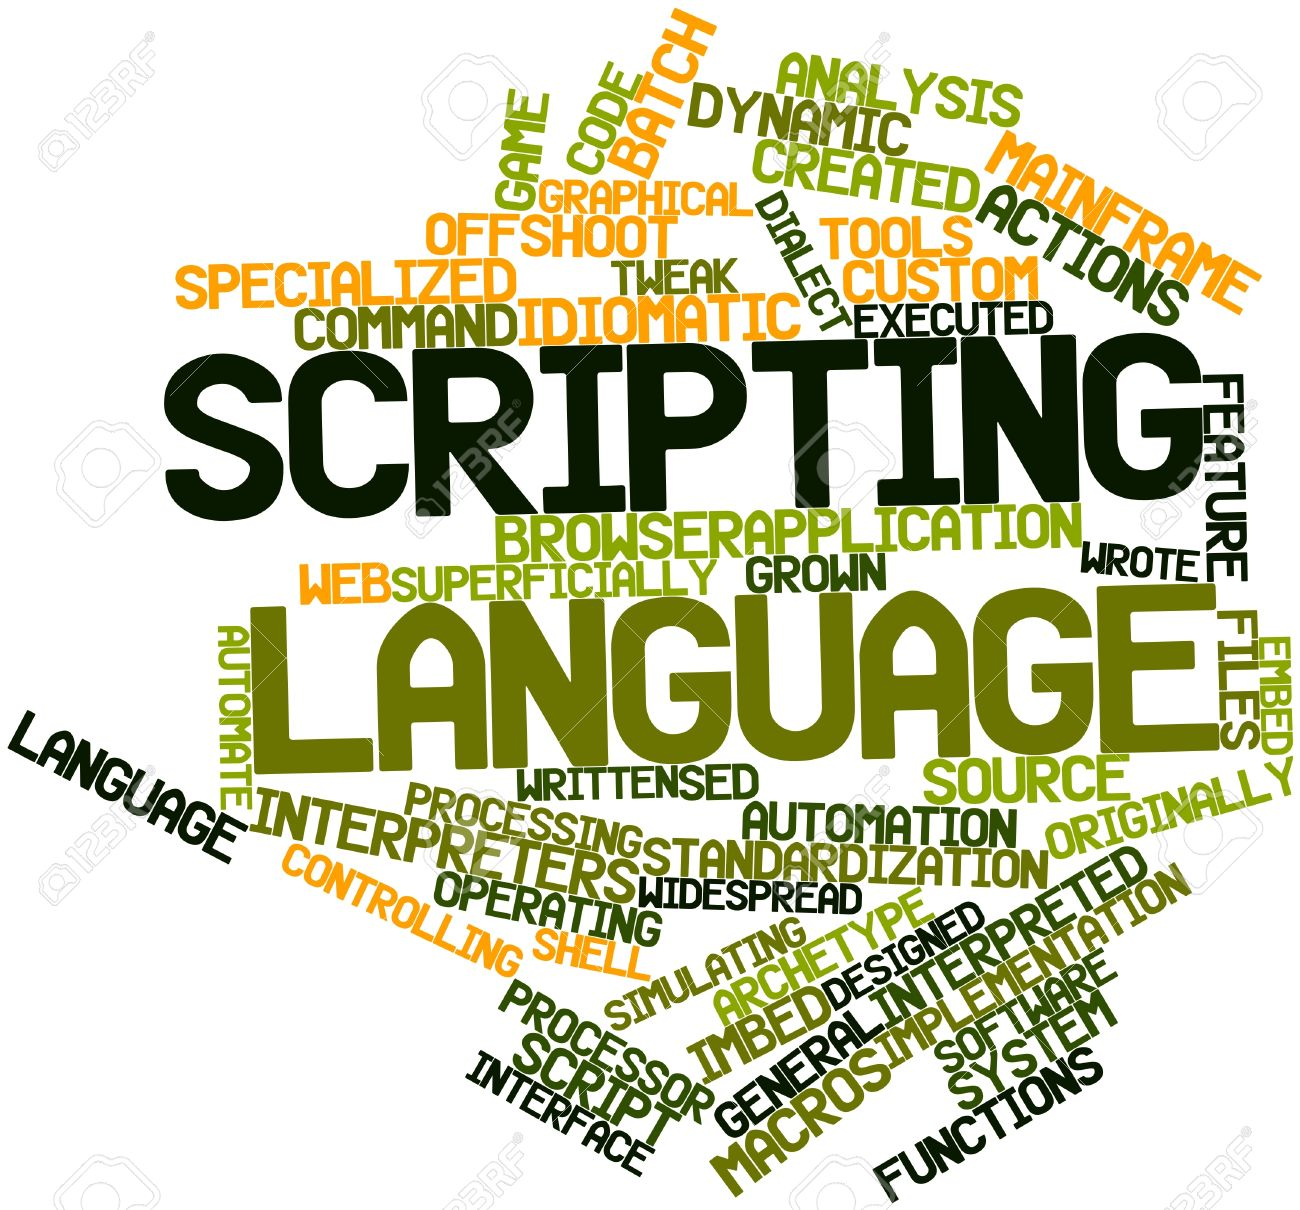
\includegraphics[scale=0.07]{res/scripting}
	\end{figure}

\end{frame}
	\iffalse
Possiamo quindi confrontare PICAT con Python. Sono stati entrambi progettati per essere linguaggi di scripting, dinamicamente tipati e permettono side effects. Una delle prime differenze è che anche se previsti PICAT scoraggia l'utilizzo di quest'ultimi mentre in Python ci sono anche funzioni built-in che fanno side effects. Ci sono poi altre differenze tra questi due linguaggi: Python è object oriented a differenza di PICAT che al massimo prevede le strutture, è differente la gestione di liste e array ed inoltre quando un programma PICAT viene compilato, cicli e list comprehension sono trasformati in chiamate tail recoursive in modo da rendere il programma più efficiente, cosa che invece Python non fa
\fi

\begin{frame}{PICAT vs Python}

	\begin{columns}

		\begin{column}{1\textwidth}

			Analogie
			\begin{itemize}
				\item Entrambi pensati come linguaggi di scripting
				\item Dinamicamente tipati
				\item Side effects
			\end{itemize}

			Differenze
			\begin{itemize}
				\item In PICAT l'uso dei side effects è scoraggiato
				\item Python è object oriented a differenza di PICAT
				\item In Python ci sono solo array dinamici mentre in PICAT abbiamo liste e array (non dinamici)
				\item In Python non è supportata l'ottimizzazione con tail recursion
			\end{itemize}

		\end{column}

		\begin{column}{0.1\textwidth}
			\begin{figure}
				\vspace*{-5cm}
				\hspace*{-2cm}
				
\includegraphics[scale=0.5]{res/pythonLogo}
			\end{figure}
		\end{column}

	\end{columns}


\end{frame}
	\iffalse
PICAT presenta alcuni vantaggi e alcuni svantaggi. Prima di tutto è di sicuro un linguaggio molto potente per la soluzione di problemi con vincoli grazie ai moduli già implementati. Possiamo fare un confronto tra un programma PICAT per la soluzione del sudoku usando il modulo cp e un programma C che risolve la stessa istanza
Altro vantaggi di PICAT è che essendo molto simile a molti altri linguaggi e poichè si può programmare in vari stili diciamo differenti è possibile fin da subito programmare qualcosa
\fi

\begin{frame}{Pro}

	\begin{columns}

		\begin{column}{1\textwidth}

			\begin{itemize}
				\item Molto efficiente se scelto bene il risolutore nella programmazione con vincoli*
				\item Essendo pensato come linguaggio di scripting molte funzioni sono già pronte
				\item Essendo multiparadigma e simile a molti altri linguaggi l'approccio iniziale è meno difficile
				\item Tabling
			\end{itemize}

		\end{column}

		\begin{column}{0.1\textwidth}
			\begin{figure}
				\vspace*{-5cm}
				\hspace*{-1.5cm}
				
\includegraphics[scale=0.3]{res/pro}
			\end{figure}
		\end{column}

	\end{columns}

\end{frame}
	\iffalse
PICAT presenta anche alcuni lati negativi dal mio punto di vista
Prima non mi piace la scelta del dinamicamente tipato, dal momento è sconsigliato l'uso di side effects e poichè non è possibile definire nuovi tipi a mio avviso potrebbe aver senso avere un controllo da parte del compilatore dei tipi
Una delle particolarità di PICAT è la possibilità di utilizzare le mappe globali. Queste possono essere sì utili ma un uso intesivo secondo me va contro una buona programmazione
Se da un lato il fatto che prenda spunto da vari altri linguaggi di programmazione può essere un aiuto per iniziare dall'altro uno può chiedersi se serviva effettivamente un altro linguaggi di programmazione. Soprattutto quando si parla di programmazione logica, per esempio, questo linguaggio è veramente molto simile al prolog.
Infine, un aspetto negativo che non è proprio del linguaggio ma ne è inevitabilmente collegato è che poichè non è molto conoscito come linguaggio si trova poco codice, poche informazioni, poche persono che lo utilizzano è questo è un problema se si vuole studiarlo a fondo
\fi

\begin{frame}{Contro}

	\begin{columns}

		\begin{column}{1\textwidth}

			\begin{itemize}
				\item Dinamicamente tipato
				\item Non ha la possibilità di dichiarare variabili costanti anche se viene sconsigliato l'uso dei side effects
				\item Global maps possono essere abusate facilmente rendendo inutile per esempio il passaggio dei parametri
				\item Molto simile ad altri linguaggi di programmazione già esistenti
				\item Scarsa documentazione e non esiste una comunità che lo utilizza
			\end{itemize}

		\end{column}

		\begin{column}{0.1\textwidth}
			\begin{figure}
				\vspace*{-5cm}
				\hspace*{-1.5cm}
				
\includegraphics[scale=0.3]{res/contro}
			\end{figure}
		\end{column}

	\end{columns}

\end{frame}
	\begin{frame}{Riferimenti}

	\begin{itemize}
		\item Constraint solving and planning with Picat, N.F. Zhou, H. Kjellerstrand, J. Fruhman
		\item My First Look At Picat as a Modeling Language or Constraint Solving and Planning, H. Kjellerstrand
		\item Documentazione Picat
		\item Picat user's Guide
		\item http://www.hakank.org/picat/
		\item https://it.wikipedia.org/wiki/Picat
		\item http://picat-lang.org/
		\item Neng-Fa Zhou - Programming in Picat https://www.youtube.com/watch?v=pQi9IPr0MFY
	\end{itemize}
	
\end{frame}
\end{document}